\chapter{Theoretical Background}


In this chapter, theoretical background of this project will be introduced in details. To better introduce the importance of the filtering, a big picture of the pipeline of tractography will be first presented. 

\section{Diffusion MRI}

Diffusion MRI is a non-invasive method to track the random microscopic motion (or diffusion) of water molecules in biological tissues. 
As molecules interact with different obstacles as they diffuse throughout tissues, 
dMRI provides insight into the microscopic details of tissue architecture \cite{newmanChapterMorphologicalBrain2014}. 
The water molecules moving in the brain tissues may cross or interact with many tissue components such as cell membranes, fibres and macromolecules. \cite{lebihanLookingFunctionalArchitecture2003}
It means the movement of these water molecules is impeded by the tissues. 
Compared to the water molecules that can move freely, 
the diffusion distance of constraint molecules is reduced and disobeys the standard 3-dimentinal Gaussian. 
This phenomenon is described in more details in the \ref{sec:dmri} as well.

\section{Fibre Orientation}
By measuring the diffusion signal, the orientations of fibres can be interpreted, and they provide the density information of the tissue of interest.
Then in the next step, the local orientation information can be pieced together to infer the long-range pathways connecting distant regions of the brain \cite{lebihanLookingFunctionalArchitecture2003}, 
which is realized with tractography. 
Currently, diffusion tensor imaging (DTI) is still the most widely used method for assessing WM orientation and organization \cite{basserEstimationEffectiveSelfDiffusion1994}.
However, when meeting more complex structures such multiple fibres crossing or passing each other, the tractography based on DTI is prone to 
generate implausible results. Therefore, to achieve better tractograms from tracking algorithms, it's essential to have diffusion model that can 
well represent the orientations. Various methods have been purposed to assess the orientations from diffusion signals, which are introduced in \ref{sec:dmri}.
In this section, methods for estimating the distribution of fiber orientations within a voxel and the high angular resolution diffusion imaging (HARDI) protocol, are explained. 

\subsection{The fibre orientation density function}
To compute the fibre orientation density function from on the measured signal, several important assumptions are made based on the characteristics of neural fibres and the diffusion inside them. 

As it introduced in the first chapter, the water molecules inside the fibres are less likely to visit other regions. First, it is assumed that there is 
no spatial exchanges between fibre bundles of different orientations. Ideally, the measured diffusion-weighted signal is formed by adding
independent signal from each area. For the curve fibres, the second assumption is made that there is no exchange between different sections of the same fibre, because
the sections will be separated by more than the diffusion distance. Therefore, the measured diffusion-weighted signal can be approximated by the sum of signals from 
different areas.

Third, different diffusion characteristics of the all fibre populations are assumed to be identical, so that the diffusion-weighted signal attenuation 
from a single oriented fibre population can be represented by an axially symmetric response function $R(h)$, where $h$ is the elevation angle in spherical coordinates \cite{tournierDirectEstimationFiber2004}. 
So the attenuation signal $S(\theta, \phi)$ measured from all fibre population can be represented by a linear combination of multiple response functions with their weights and rotation, which is written as:

\begin{gather}\label{attenuationsignal}  
    S(\theta, \phi) = \sum_{i}^{}f_{i}\hat{A}_{i}R(\theta)
\end{gather}

In the equation\ref*{attenuationsignal},  $f_{i}$ is the volume fraction for the $i$th fiber population, and $\hat{A}_{i}$ is the operator representing a rotation onto the direction $\theta_{i}, \phi_{i}$ \cite{tournierDirectEstimationFiber2004}.
This equation can also be expressed by a convolution of a unit sphere of response function with the fibre density distribution function(fODF), which is written as:

\begin{gather}\label{convo}  
    S(\theta ,\phi ) = F(\theta ,\phi ) \otimes R(\theta)
\end{gather}

The fODF gives the volume fraction of the fibres that have the same orientation $(\theta, \phi)$ expressed in spherical coordinates. 
If there are $n$ distinct fibre population, then fODF consists of $n$ Dirac delta functions indicating the orientations and the respective weights
from the volume fractions. An example when $n = 2$ is given below in Fig \ref{fig:2dconv}. 

\begin{figure}[ht]
    \centering
    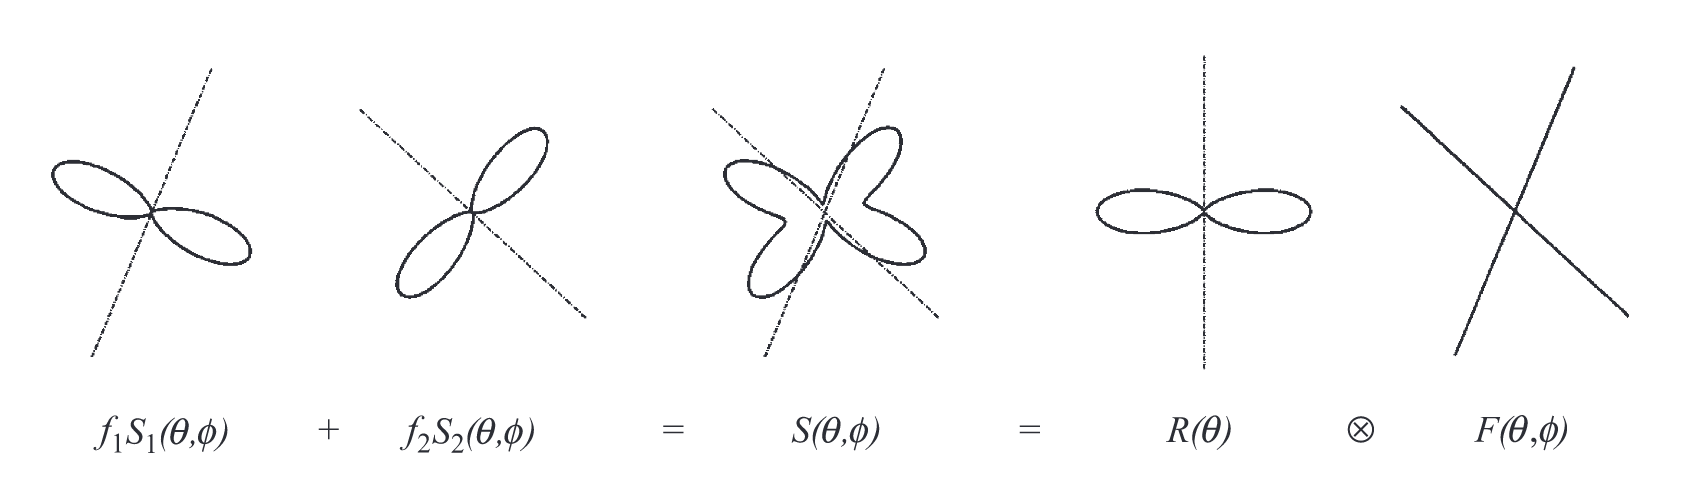
\includegraphics[width= 15cm]{figures/2D.png}
        \caption{In this simple 2D illustration, the voxel contains two fiber populations with distinct orientations
         $(\theta_{1} ,\phi_{1})$ and $(\theta_{2} ,\phi_{2})$, and volume fractions $f1$ and $f2$ ($f1 = f2 = 1/2$ in this case). 
         For each plot, the dotted lines represent the fiber orientation(s) and the continuous line the corresponding signal attenuation. 
         The measured diffusion-weighted signal attenuation $S(\theta, \phi)$ is the sum of each fiber population’s characteristic profile $S_{1}(\theta, \phi) = \hat{A}_{1}R(\theta)$, and $S_{2}(\theta, \phi) = \hat{A}_{2}R(\theta)$, 
         weighted by their respective volume fractions. This can be expressed as a convolution over the unit sphere of an axially symmetric response function R(h), 
         describing the signal attenuation measured for a single fiber population, with a fiber orientation density function $F(\theta ,\phi)$, 
         describing the fiber orientations present in the voxel \cite{tournierDirectEstimationFiber2004}. }
    \label{fig:2dconv}
\end{figure}

\subsection{HARDI}
High angular resolution diffusion imaging (HARDI) is a type of dMRI that measures diffusion signals on a sphere in q-space \cite{consagraOptimizedDiffusionImaging2022}.
During the scanning of high-angular resolution, the signal $S(\theta, \phi)$ is collected in a great number of orientations.
So the white matter structure is estimated by constructing fODF. Spherical deconvolution (SD) is used to estimate fODF in each brain voxel. 
The original diffusion weighted signal is formed from the
various fibre population, and given by spherical convolution of the response functions with the fODF (the apparent density of fibres as a function of orientation) \cite{jeurissenMultitissueConstrainedSpherical2014}. 
If the $R(\theta)$ is known, the fODF can be obtained by the SD of the response function from the measured DW signal inversely.
\subsection{Spherical Deconvolution}
Spherical function is usually represented by a linear combination of spherical harmonics and rotational harmonics. 
The spherical harmonics form a complete orthonormal basis set of functions over the sphere, 
much like the Fourier series forms a complete orthonormal basis over an interval in Cartesian space \cite{tournierDirectEstimationFiber2004}.
Each spherical harmonic contains two main parameters: its order $n$ ($n \geq  0$) and phase factor $m$ ($ -n \leq m \leq n$). 
Increasing order $n$ indicates the higher angular frequency. 

The spherical convolution process is regarded as an action which contains a series of rotation on a function defined over a sphere, which can be related
to the equation \ref{attenuationsignal}. If $\underline{F}^{n}$ is defined to be a vector containing $2n+1$ harmonics in $n$th order 
and $R_{n}$ is the matrix of size $(2n+1)(2n+1)$ representing the $n$th order of rotational harmonics, 
so the $n$th order spherical representation of $S(\theta, \phi)$ can be expressed as:

\begin{gather}\label{sc}  
    S^{n} = R^{n} \underline{F}^{n}
\end{gather}
Therefore, the spherical deconvolution operation can be performed simply by inverting each $R^{n}$ matrix to recover $\underline{F}^{n}$. 

\subsection{Constrained Spherical Deconvolution}
Obtaining the unknown coefficients of fODF through the deconvolution operation on the spherical convolution matrix can be cast as a linear least-squares problem \cite{jeurissenMultitissueConstrainedSpherical2014}.
But this operation can be sensitive to noise and ill-posed. Thus, the constraint SD (CSD) is purposed which performs the SD operation with drastically reduced noise sensitivity, 
allowing reliable fODF estimates on clinically feasible DW-MRI data \cite{tournierRobustDeterminationFibre2007}. CSD performs well in pure WM, while it's prone to produce 
noise in grey matter (GM) and cerebrospinal fluid (CSF) \cite{jeurissenMultitissueConstrainedSpherical2014}. 

So another technique named multi-shell, multi-tissue CSD (MSMT-CSD) is purposed, which assumes that the DW signal arises from the contributions of the three main tissue types found in the brain: WM, GM and CSF \cite{jeurissenMultitissueConstrainedSpherical2014}.
Using MSMT-CSD, the ODF of WM is considered to be anisotropic, while in GM and CSF the ODF is considered to be isotropic and uses an SH series of order 0. 
Some study has shown that compared to single shell single tissue CSD (SSST-CSD), MSMT-CSD can substantially increase the precision of the fODF fibre orientations 
and reduce the presence of spurious fODF peaks in voxels containing GM and/or CSF \cite{jeurissenMultitissueConstrainedSpherical2014}.

\section{Tractography}

Test \autocite{dhollanderFixelbasedAnalysisDiffusion2021}


\section{Fibre Filtering Methods}

\subsection{COMMIT}

\subsubsection{Filtering Theory}

\subsubsection{Existing Problems}

\subsection{SIFT}

\subsubsection{Filtering Theory}

\subsubsection{Filtering Theory}

\section{Deep Learning Based Classification}

\subsection{Multiple Layer P}
\subsection{RNN}




